
\chapter{Introduction: Imbalanced Classification Learning}

%\setlength{\epigraphwidth}{3.5in} 
%\epigraph{\textit{``Most people do not listen with the intent to understand; they listen with the intent to reply."} --- Stephen R Covey}

%Artificial intelligence (AI), powered by machine learning (ML), is transforming the world we live in today. 
%AI and ML applications which were previously limited to constrained environments are nowadays widely deployed in almost every field in the wild. 
%ML techniques are broadly classified intro two categories based on the nature of output random variable.
%Firstly, classification models deal with discreet random variables and hence model categorical distributions. 
%Lastly, regression models deal with continuous random variables hence model continuous distributions.
Machine learning (ML) based classifiers have numerous applications in real world; e.g., spam email detection, cancerous tumor detection, fraudul transaction detection, text sentiment analysis and emotion analysis, image classification and object detection, named entity recognition and information extraction.
Classifiers are usually studied under balanced categorical distributions (BCD) for simplicity; many datasets curated and used by academia have balanced categories. %\footnote{Many text classification datasets made accessible via huggingface-datasets, tensorflow-datasets and torchtext are purposefully balanced: e.g. even though DBpedia ontology classes are imbalanced in nature, the commonly used DBpedia-14 dataset is balanced.},
%e.g., SNLI \cite{maccartney-manning-2008-snli}, Sentiment Classification (IMDb reviews) \cite{maas-etal-2011-imdbreview}, MultiNLI \cite{williams-etal-2018-multinli}, XNLI \cite{conneau-etal-2018-xnli}, CIFAR-\{10,100\} \cite{Krizhevsky-2009-CIFAR}, nearly balanced, e.g. MNIST \cite{lecun1998-mnist}.
However, naturally occurring categorical distributions are often imbalanced. 
In many real-world settings, imbalance is inevitable, e.g. fewer cancerous patients than non-cancerous, fewer fraud transactions than legit, spam and ham mails are not evenly distributed.
And in some scenarios balancing is impossible; e.g. image segmentation task has more background pixels than the foreground pixels, and in natural languages, the each stopword type has more tokens than each content type.
An imbalanced categorical distribution (ICD) results in the formation of majority and minority categories.\footnote{
The terms \textit{majority} and \textit{minority} may sometimes be referred as \textit{frequent} and \textit{rare}, respectively. The term \textit{category} is referred as \textit{class} in the context of machine learning, as \textit{group} in social sciences, \textit{symbol} in symbolic communication systems, and as \textit{type} in the context of natural language processing.} 
The minority categories are at least as important, if not more, as majority categories. 

When ML classification techniques are applied on imbalanced distributions without accounting for the imbalance, we face the following two problems:
\begin{enumerate}
\item There exist noticeable performance difference between majority and minority classes. 
% The difference varies based on the level of imbalance. 
Classifiers achieve higher performance (usually quantified using F-measure) on the majority classes whereas relatively poor performance on minority classes. 
Sometimes this phenomenon is attributed as frequency-based biases; specifically, minority classes suffer from under-recall, hence poor recall, and the majority classes suffer from over-recall, hence poor precision.

\item Evaluation metrics that do not consider imbalance into account, e.g, Accuracy, overlook performance on minority categories. 
Rounding the system level score to a few decimal points is a common practice which helps masking out unnecessary detail and establishing significance in the performance improvements. 
When majorities and minorities are put together without addressing the imbalance and rounded the resulting system level score to a few decimal points, the impact of minorities performance looks too small that they risk being \textit{ignored} or \textit{not significant}.
\end{enumerate}


The problem of imbalance in categorical distributions is studied in classical ML era \cite{provost2000-ml-imb-101, japkowicz2002ClassImbalance,chawla-etal-2004-special-issue}.
In the medical domain \citet{Maciej2008MedicalImbalance} find that classifier performance deteriorates with even modest imbalance in the training data.
However, with the neural networks, there is only scant effort:
Untreated class imbalance has been known to deteriorate the performance of image segmentation; 
\citet{Sudre2017GeneralizedDice} investigate the sensitivity of various loss functions.
\citet{buda-etal-2018-imbalance-cnn} investigate the impact of class imbalance on convolutional neural networks' classification performance and also conclude that class imbalance is detrimental. % definition and quantification method for two types of class imbalance: \textit{step imbalance} and \textit{linear imbalance}.
%Since the imbalance in Zipfian distribution of classes is neither single-stepped nor linear, we use a divergence based measure to quantify the imbalance.


%\textcolor{gray6}{
Though the imbalanced categorical distributions are prevalent in almost every domain, the efforts towards learning from imbalanced distributions is mostly targeted to computer vision tasks \cite{Johnson2019SurveyImbalance}.
With neural network being a universal function approximator and deeplearning becoming mainstream machine learning paradigm, the boundaries between different kinds of tasks are favorably blurred: the deeplearning models are borrowed from one domain to other: CNN models which were originally used for computer vision are now being used for natural language processing (NLP), and the Transformer models which were originally used for NLP tasks are now also being used for computer vision.
Hence, we believe the findings on imbalanced learning can also be transferrable from one domain to the other, although it is not formally verified before.

In this work, we like to take the learning from tasks where imbalanced learning is well explored and apply it to the areas such as natural language generation where the efforts are scant.
It is known that word types in natural languages resemble Zipfian distribution \cite{zipf1949human,powers-1998-zipf-apps}, which is an extremely imbalanced, long-tail distribution. 
In any natural language system, some word types occur very frequently and a vast number of types occur rarely. 
In a typical class imbalanced setting, ML models tends to have high performance on majority classes, as there are plenty of examples to learn from, while poor performance on minority classes for which there are only a limited number of examples.
In symbolic communication systems, the rare \textit{symbols} contain more \textit{information content} than frequent symbols \cite{shannon1948mathematical}.
Since natural languages are also symbolic communication systems, rare types are equally or more important than the frequent types \cite{gowda2021macroaverage}. 
The imbalance problem in language systems is particularly challenging and requires our attention due to the fact that rare types carry crucial information \cite{steedman-2008-last}.
For example, machine translation models trained have poor performance for the rare types where the crucial information is \cite{gowda-may-2020-finding,gowda2021-many-eng}.
Hence, we emphasize that extra care concerning the imbalance is necessary for the application of ML to natural language processing (NLP), and we attempt to address exactly that in this work.

We present our findings in the following order:
In Chapter \ref{ch:affirmative-action}, we describe that the objective of imbalance learning is \textit{going the extra mile} in favor of minority categories, whose parallel counterpart in the social sciences is called \textit{affirmative action} (AA), and discuss its ethical implications. 
In Chapter \ref{ch:nlg-imbalance}, we focus on (neural) machine translation (NMT), a natural language generation task and show the consequences of imbalance.
NMT is commonly not seen as classification task and class imbalance is ignored, we envision NMT model as a kind of multi-class classification task where classes are the target language vocabulary, we show that imbalance affects hyperparamaters such as vocabulary size and show that NMT models have biases resulting from class imbalance which was previously unknown.
In Chapter \ref{ch:eval-metrics}, we show that current evaluation metrics are ignorant of imbalance, and some new ones proposed are biased and opaque; we present an evaluation metric that accounts class imbalance at the testing stage.
In Chapter \ref{ch:imb-learning}, we study both the methods and our proposed methods for machine learning from imbalanced categorical distributions.
Here we consider NMT as a complex classification task, we start with simple classification tasks such as image classification, text classification and build our way to the NMT task.
In Chapter \ref{ch:applications}, by applying our simplified view of NMT as multi-classifier on the target language, we develop many-to-one translation model. While current multilingual NMT efforts are limited to 100 languages, we push its limits with 500 to English translation (i.e. 4 times more source languages). 


\begin{figure}[ht]
    \centering
    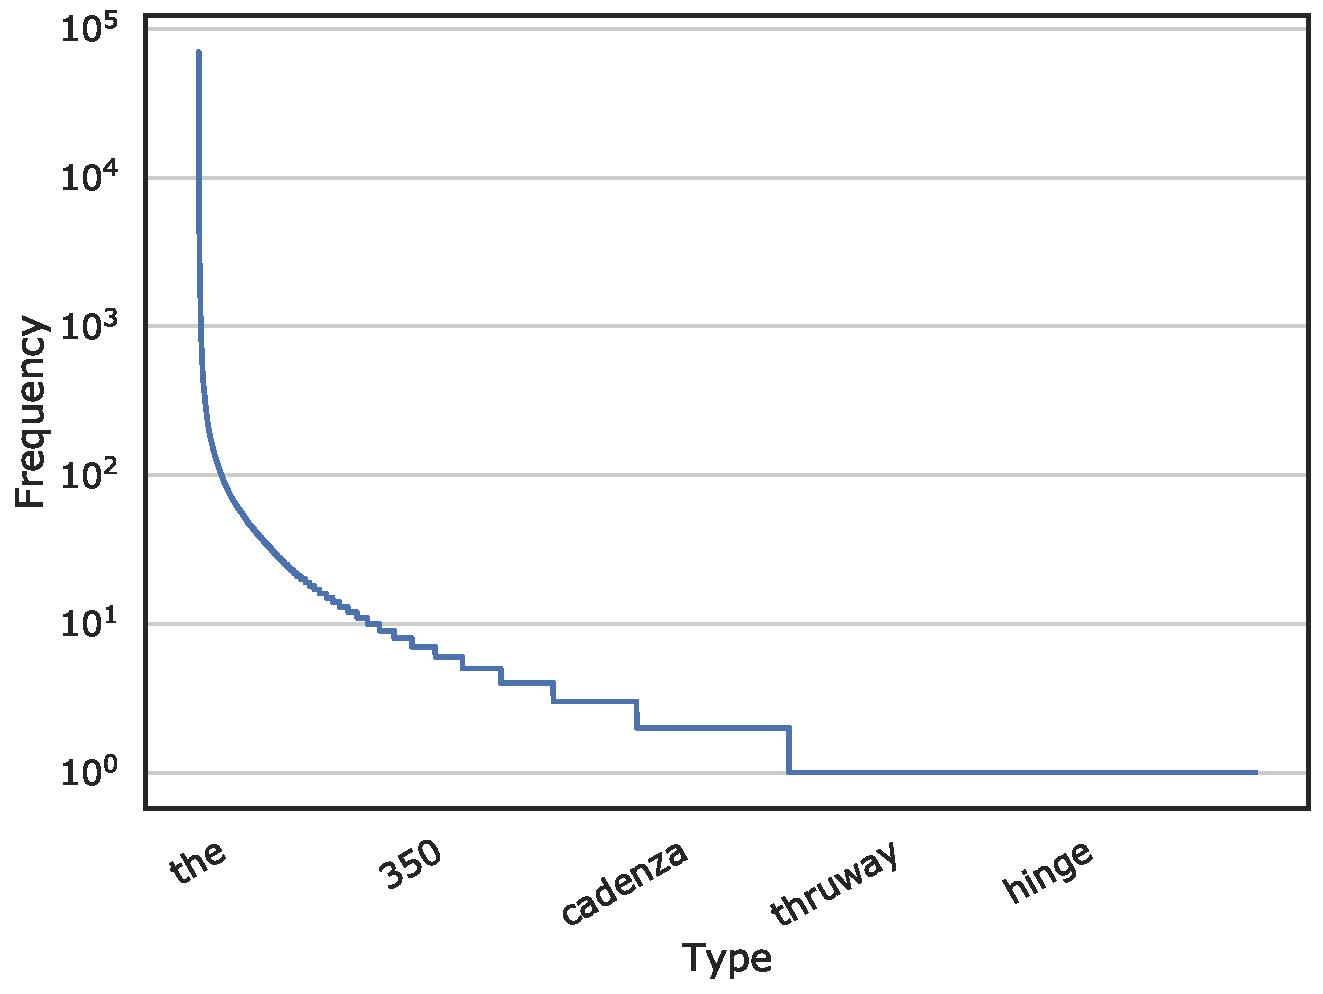
\includegraphics[width=0.75\textwidth]{img/background/brown-corpus-zipf.pdf}
    
    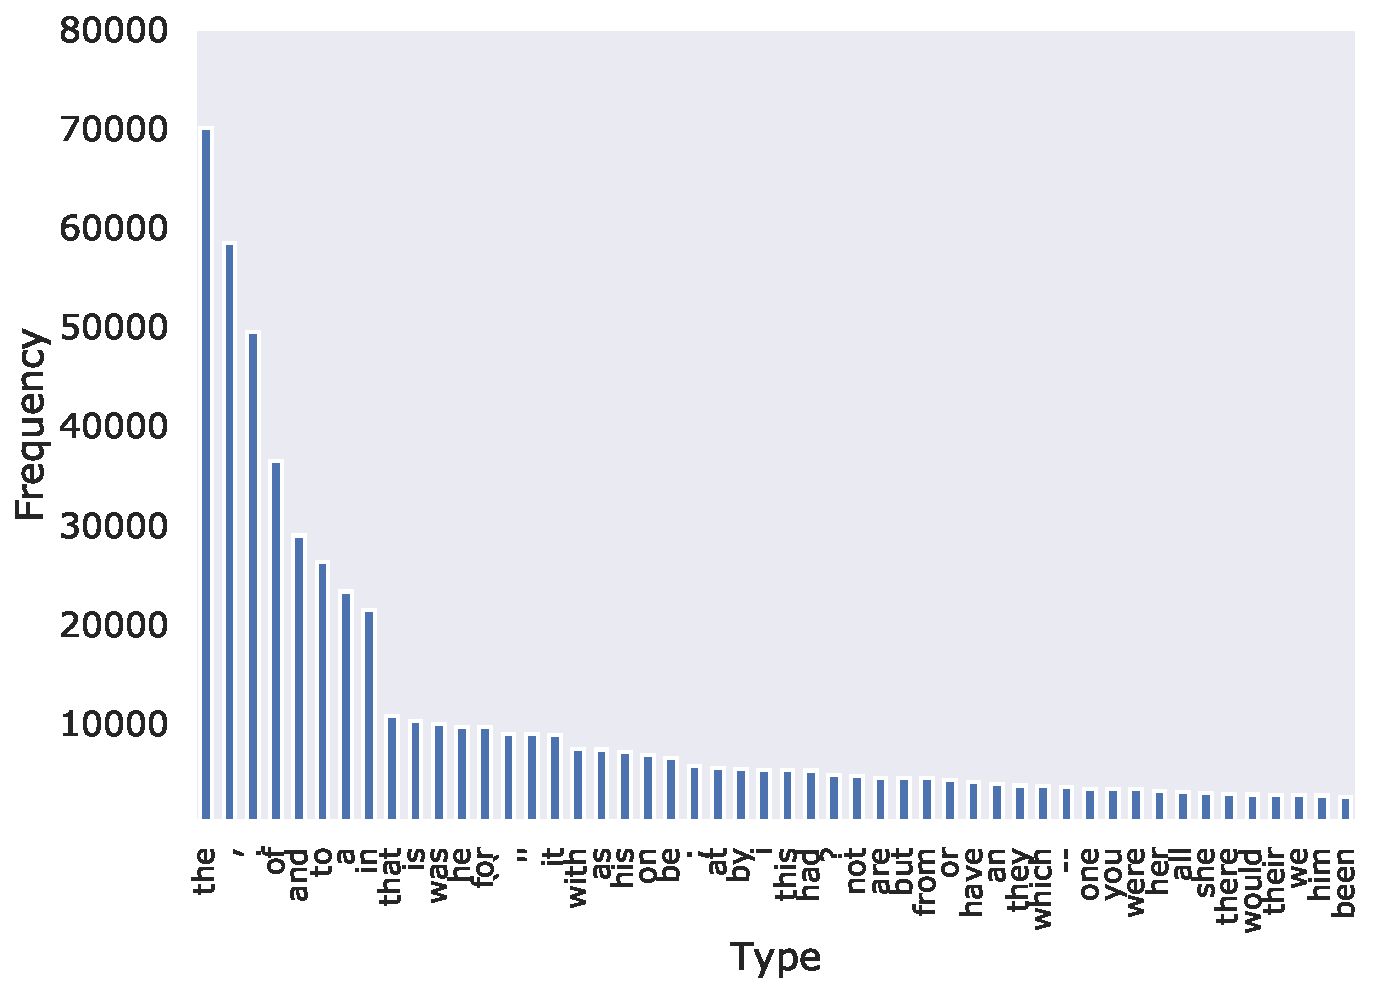
\includegraphics[width=0.75\textwidth]{img/background/brown-corpus-zipf-top50.pdf}
    \caption{Caption}
    \label{fig:my_label}
\end{figure}
\begin{figure}[ht]
    \centering
    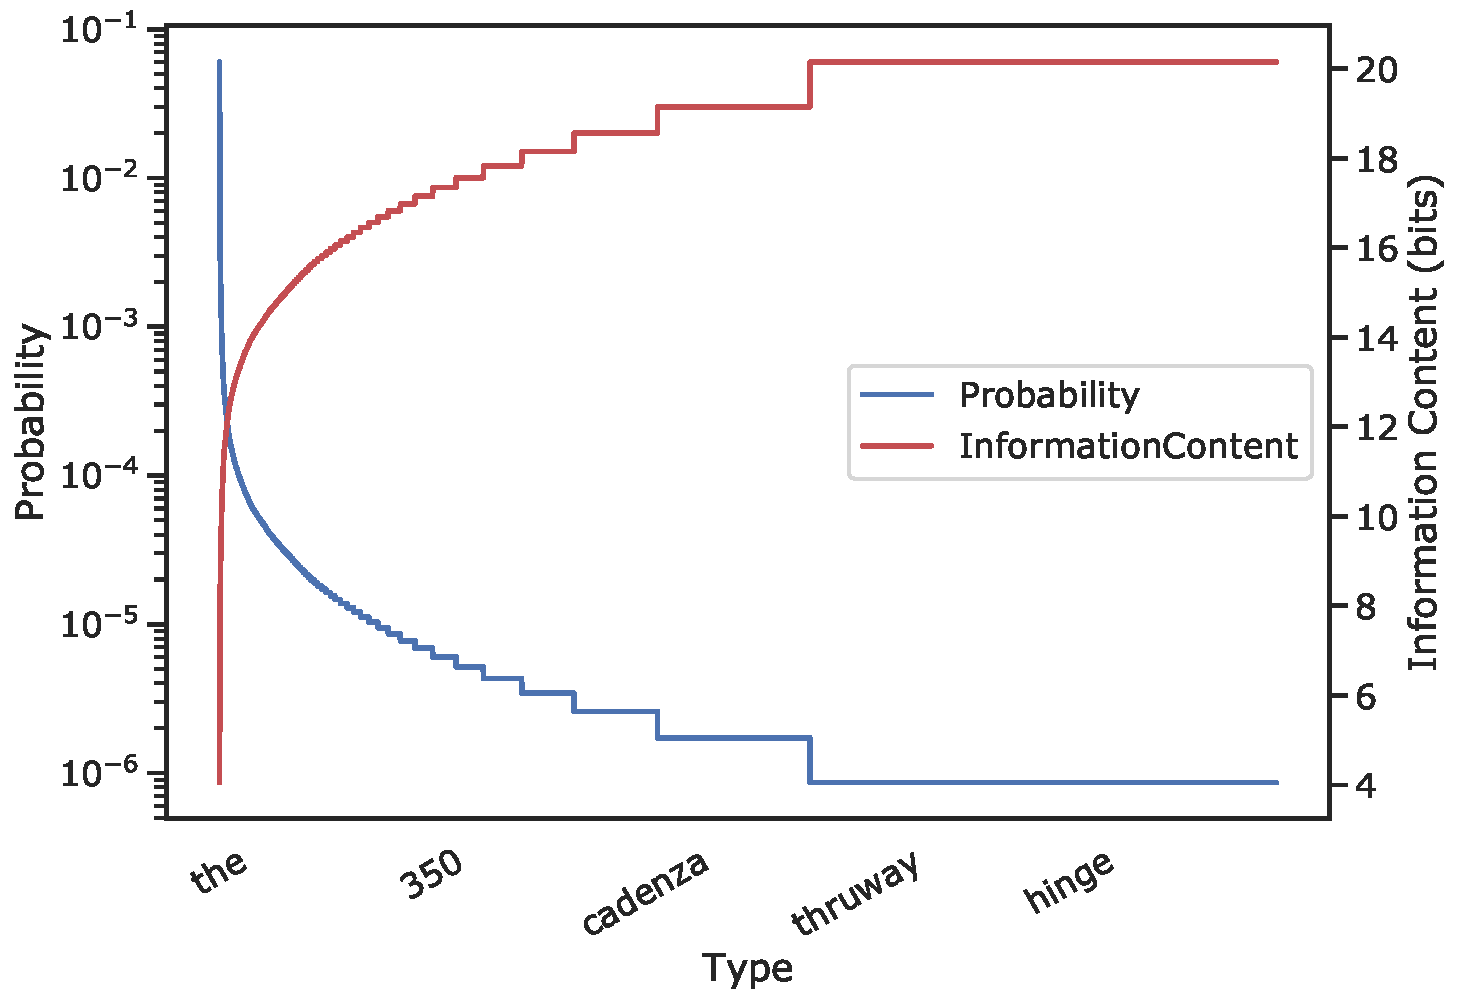
\includegraphics[width=0.75\textwidth, trim={3mm 0 3mm 0}, clip] {img/background/brown-corpus-shannons.pdf}
    \caption{Caption}
    \label{fig:my_label}
\end{figure}


%%---- COMMENT -----
\begin{comment}
Consider rare type translation: when the source and the target languages use the same alphabet,
%e.g. Romance languages such as English, French, Spanish, German, etc,
the rare types such as proper nouns and numeric types are often cognates which can be simply copied from the source to the target side without translation or transliteration. 
Shared vocabulary with tied embeddings which is widely used in the current translation models exploit this phenomenon ~\cite{press-wolf-2017-embeddings,vaswani2017attention}.
However, when translating between languages of heterogeneous scripts, rare word translation is more problematic.
Though techniques such as byte-pair-encoding \cite{sennrich-etal-2016-bpe} alleviate this problem, it is not entirely resolved ~\cite{gowda-may-2020-finding}.

\begin{figure}
    \centering
    \includegraphics[width=\linewidth]{img/gtranslate-error2.png}
    \caption{An example error from Google Translate {\footnotesize (accessed: June 15, 2021)}: `984' (in Kannada script) is translated to `2' in English; `984' is the crucial information in this example sentence.}
    \label{fig:gtrans-err}
\end{figure}
\end{comment}

%%---- COMMENT -----

\textbf{Proposal:} We propose to study and advance the following research arenas:
\begin{enumerate}
 \item How is class imbalance affecting NLG?
 \item Are the current NLG evaluation metrics addressing class imbalance? If not, how to create a metric that address imbalance?
 \item How to improve NLG performance in the light of imbalance?
\end{enumerate}

%We aim to study imbalanced learning under the realm of neural machine translation (NMT) task, however, since classifier is entangled with an autoregressor in NMT, certain imbalance learning strategies such as over-sampling and under-sampling are not directly applicable. 
%Imbalanced learning is widely studied under clearly defined classification tasks such as image classification. 